% The device kernels' thread mappings: a thread per element for the element stores of TET4, TET10 and
% HEX8 (atomic or block-local scatter), a thread per quadrature point for the HEX27 point store, a warp
% per element for the HEX27 element matrix, and a thread per row of SELL-32 slices for the quantized
% matrix.
\documentclass[border=2pt]{standalone}
% Shared preamble of the format diagrams: colours of the paper's figures (paper_figures.py) and
% the drawing styles.  Each diagram is a standalone document built to a PDF of the text width.
\usepackage{amsmath,amssymb}
\usepackage{tikz}
\usetikzlibrary{arrows.meta,calc,decorations.pathreplacing,patterns,positioning}

\definecolor{cindex}{HTML}{BDBDBD}  % column indices, offsets, row pointers
\definecolor{cvalue}{HTML}{6E6E6E}  % floating-point values (BSR)
\definecolor{cpoint}{HTML}{1B9E77}  % quadrature-point store
\definecolor{celem}{HTML}{1F78B4}   % element matrix
\definecolor{cqbsr}{HTML}{A6761D}   % quantized BSR
\definecolor{cscale}{HTML}{E6AB02}  % scales
\definecolor{cmean}{HTML}{7570B3}   % f32 element mean

\tikzset{
  >={Stealth[length=4pt]},
  grid/.style={draw=black!45, line width=0.25pt},
  frame/.style={draw=black!70, line width=0.5pt},
  title/.style={font=\small\bfseries, anchor=west, inner sep=0pt},
  lab/.style={font=\footnotesize, inner sep=1pt},
  note/.style={font=\scriptsize, text=black!75, inner sep=1pt, execute at begin node={\hyphenpenalty=10000\exhyphenpenalty=10000}},
  num/.style={font=\tiny, inner sep=0pt},
  brace/.style={decorate, decoration={brace, amplitude=3pt, raise=1pt}, line width=0.4pt},
  arr/.style={->, line width=0.5pt, black!70},
  pad/.style={pattern=north east lines, pattern color=black!30},
}

% \cell{x}{y}{w}{h}{fill}: a filled rectangle with a thin outline, lower-left corner at (x,y).
\newcommand{\cell}[5]{\filldraw[fill=#5, grid] (#1,#2) rectangle ++(#3,#4);}
% \blk{x}{y}{s}{fill}: a 3x3 block of side s with its 3x3 entry grid.
\newcommand{\blk}[4]{%
  \filldraw[fill=#4, grid] (#1,#2) rectangle ++(#3,#3);
  \draw[draw=white, line width=0.25pt] (#1,#2) ++(#3/3,0) -- ++(0,#3) ++(#3/3,0) -- ++(0,-#3);
  \draw[draw=white, line width=0.25pt] (#1,#2) ++(0,#3/3) -- ++(#3,0) ++(0,#3/3) -- ++(-#3,0);
  \draw[grid] (#1,#2) rectangle ++(#3,#3);}
% \vthree{x}{y}{fill}: a 3-vector (one node's components) as three small cells, left end at (x,y).
\newcommand{\vthree}[3]{\foreach \k in {0,1,2} \filldraw[fill=#3, grid] (#1+\k*0.14,#2) rectangle ++(0.14,0.14);}
% \op{x}{y}{symbol}: an operation in a small circle.
\newcommand{\op}[3]{\node[circle, draw=black!70, line width=0.4pt, inner sep=0.5pt, minimum size=9pt, font=\tiny] at (#1,#2) {#3};}

\begin{document}
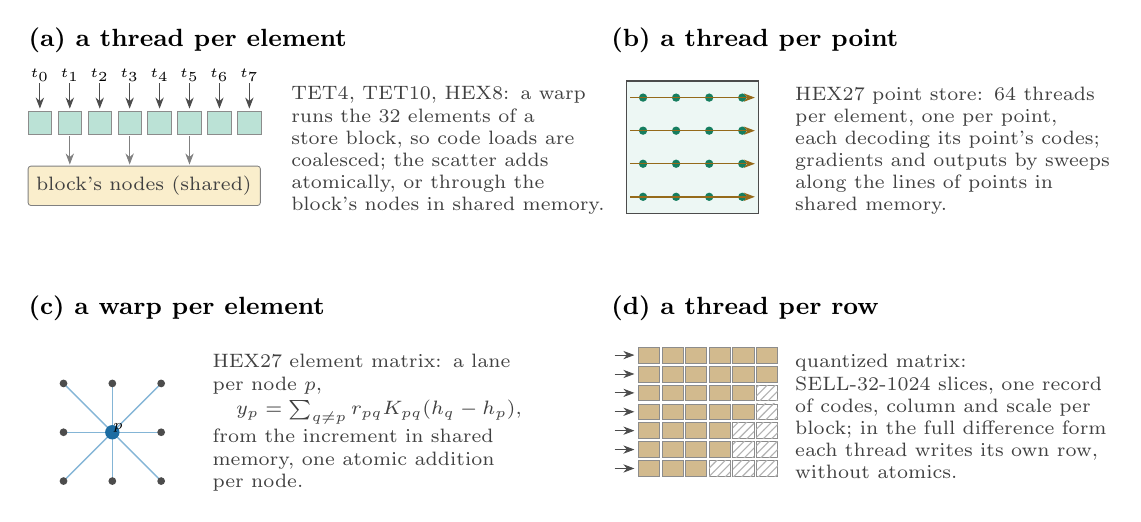
\begin{tikzpicture}
  \tikzset{
    expl/.style={note, anchor=north west, align=left, text width=4.0cm},
  }
  % ---------------------------------------------------------------- (a) a thread per element
  \begin{scope}[shift={(0,3.4)}]
    \node[title] at (0, 2.75) {(a) a thread per element};
    \foreach \l in {0,...,7} {
      \filldraw[fill=cpoint!30, grid] (\l*0.38,1.55) rectangle ++(0.3,0.3);
      \draw[arr, line width=0.35pt] (\l*0.38+0.15,2.2) -- (\l*0.38+0.15,1.88);
      \node[num] at (\l*0.38+0.15,2.3) {$t_{\l}$};
    }
    \filldraw[fill=cscale!20, draw=black!50, line width=0.3pt, rounded corners=1pt] (0.0,0.65) rectangle (2.95,1.15);
    \node[note] at (1.47,0.9) {block's nodes (shared)};
    \foreach \l in {1,3,5} \draw[arr, line width=0.3pt, black!50] (\l*0.38+0.15,1.53) -- (\l*0.38+0.15,1.17);
    \node[expl] at (3.3,2.2) {TET4, TET10, HEX8: a warp runs the $32$ elements of a store block, so code loads are coalesced; the scatter adds atomically, or through the block's nodes in shared memory.};
  \end{scope}

  % ---------------------------------------------------------------- (b) a thread per point (HEX27)
  \begin{scope}[shift={(7.4,3.4)}]
    \node[title] at (0, 2.75) {(b) a thread per point};
    \def\s{0.42}
    \filldraw[fill=cpoint!8, frame] (0.2,0.55) rectangle ++(4*\s,4*\s);
    \foreach \i in {0,...,3} \foreach \j in {0,...,3}
      \node[circle, fill=cpoint!80!black, inner sep=0pt, minimum size=3pt] at ({0.2+(\i+0.5)*\s},{0.55+(\j+0.5)*\s}) {};
    \foreach \j in {0,...,3} \draw[arr, cqbsr!90!black, line width=0.5pt] (0.25,{0.55+(\j+0.5)*\s}) -- ({0.15+4*\s},{0.55+(\j+0.5)*\s});
    \node[expl] at (2.3,2.2) {HEX27 point store: $64$ threads per element, one per point, each decoding its point's codes; gradients and outputs by sweeps along the lines of points in shared memory.};
  \end{scope}

  % ---------------------------------------------------------------- (c) a warp per element (HEX27)
  \begin{scope}[shift={(0,0)}]
    \node[title] at (0, 2.75) {(c) a warp per element};
    \def\s{0.62}
    \foreach \i in {0,...,2} \foreach \j in {0,...,2} \coordinate (n\i\j) at ({0.45+\i*\s},{0.55+\j*\s});
    \foreach \i in {0,...,2} \foreach \j in {0,...,2} {\ifnum\i\j=11 \else \draw[celem!55, line width=0.5pt] (n11) -- (n\i\j); \fi}
    \foreach \i in {0,...,2} \foreach \j in {0,...,2} \fill[black!70] (n\i\j) circle (1.4pt);
    \fill[celem!90!black] (n11) circle (2.6pt);
    \node[num, anchor=south west] at (n11) {$p$};
    \node[expl] at (2.3,2.2) {HEX27 element matrix: a lane per node $p$,\\[1pt] \hspace*{0.3cm}$y_p=\sum_{q\ne p} r_{pq}K_{pq}(h_q-h_p)$,\\[1pt] from the increment in shared memory, one atomic addition per node.};
  \end{scope}

  % ---------------------------------------------------------------- (d) a thread per row (quantized matrix)
  \begin{scope}[shift={(7.4,0)}]
    \node[title] at (0, 2.75) {(d) a thread per row};
    \def\w{0.3}\def\h{0.2}
    \foreach \len [count=\i from 0] in {6, 6, 5, 5, 4, 4, 3} {
      \pgfmathsetmacro{\y}{2.05-\i*(\h+0.04)}
      \foreach \k in {0,...,5} {
        \pgfmathsetmacro{\x}{0.35+\k*\w}
        \ifnum\k<\len \filldraw[fill=cqbsr!50, grid] (\x,\y) rectangle ++(\w-0.03,\h);
        \else \filldraw[fill=white, grid] (\x,\y) rectangle ++(\w-0.03,\h); \fill[pad] (\x,\y) rectangle ++(\w-0.03,\h); \fi
      }
      \draw[arr, line width=0.3pt] (0.05,\y+\h/2) -- (0.3,\y+\h/2);
    }
    \node[expl] at (2.3,2.2) {quantized matrix: SELL-$32$-$1024$ slices, one record of codes, column and scale per block; in the full difference form each thread writes its own row, without atomics.};
  \end{scope}
\end{tikzpicture}
\end{document}
